\documentclass[12pt,aspectratio=169]{beamer}

\usetheme[progressbar=frametitle, numbering=fraction]{metropolis}
\usepackage{appendixnumberbeamer}
\usepackage{gensymb}
\usepackage{booktabs}
\usepackage[scale=2]{ccicons}

\usepackage{pgfplots}
\usepgfplotslibrary{dateplot}
\usepackage[english]{babel}

\usepackage{xspace}
\newcommand{\themename}{\textbf{\textsc{metropolis}}\xspace}

\usepackage{amsmath}

% Chinese Fonts (Fontset: fandol,ubuntu)
\usepackage[fontset=windows]{ctex}

% Math Fonts
\usefonttheme{professionalfonts}
\usepackage{mathspec}
\setsansfont[BoldFont={Fira Sans},
  Numbers={OldStyle}]{Fira Sans Light}
\setmathsfont(Digits)[Numbers={Lining, Proportional}]{Fira Sans Light}

% Change Color of the theme
\usepackage{xcolor}
\definecolor{DarkGrey}{HTML}{353535}
\definecolor{ECNURed}{RGB}{164,31,53}
\definecolor{ECNUBrown}{RGB}{134,117,77}
\definecolor{BackGround}{RGB}{250,250,250}
\definecolor{MyBlue}{RGB}{0,161,233}
\definecolor{MyRed}{RGB}{228,0,127}
\setbeamercolor{normal text}{ fg= DarkGrey  }
\setbeamercolor{alerted text}{ fg= ECNURed  }
\setbeamercolor{example text}{ fg= ECNUBrown  }

% Bolder Fonts for presenting in a large room 
\setsansfont[BoldFont={Fira Sans SemiBold}]{Fira Sans}
\metroset{block=fill}

\usepackage{listings,xcolor}
\usepackage{tikz}
\usepackage{pgfmath}
\usepackage{animate,media9,graphicx}
\usepackage{calligra}
\usepackage{array}
\renewcommand{\arraystretch}{2}  % 增加行高
\setlength{\tabcolsep}{10pt}     % 增加列间距

\lstset{
  language         = c++,
  numbers          = left,
  numberstyle      = \tiny,
  breaklines       = true,
  captionpos       = b,
  tabsize          = 4,
  frame            = shadowbox,
  columns          = fullflexible,
  commentstyle     = \color[RGB]{0,128,0},
  keywordstyle     = \color[RGB]{0,0,255},
  basicstyle       = \tiny\ttfamily,
  stringstyle      = \color[RGB]{148,0,209}\ttfamily,
  rulesepcolor     = \color{red!20!green!20!blue!20},
  showstringspaces = false,
}

\title{Neural Ordinary Differential Equations}
\subtitle{}
\author{Yifei Ding}
\date{\today}
% \institute{演讲者描述}
% \titlegraphic{\hfill
\includegraphics[height=1.5cm]{ECNUlogo.png}}

\begin{document}

\maketitle
% \footnotesize
% \begin{frame}{Contents}
%   \setbeamertemplate{section in toc}[sections numbered]
%   \tableofcontents%[hideallsubsections]
% \end{frame}

\begin{frame}{Introduction}
  \[
    \textbf{\textrm{h}}_{t+1}=\textbf{\textrm{h}}_t+f(\textbf{\textrm{h}}_t,\theta_t)
    \Longrightarrow
    \frac{\textrm{d}\textbf{\textrm{h}}(t)}{\textrm{d}t}=f(\textbf{\textrm{h}}(t),t,\theta)
  \]

  \vspace{1cm}

  Benefits: memory efficiency, adaptive computation, scalable and invertible
  normalizing flows, continuous time-series models
\end{frame}

\begin{frame}{Backpropagation}
  \[
    L(\textbf{\textrm{z}}(t_1))=L\left(\textbf{\textrm{z}}(t_0)+\int_{t_0}^{t_1}
    f(\textbf{\textrm{z}}(t),t,\theta)\textrm{d}t\right)=L(\textrm{ODESolve}
    (\textbf{\textrm{z}}(t_0),f,t_0,t_1,\theta))
  \]

  \vspace{1cm}

  Target:
  \[\frac{\partial L}{\partial \theta}\]
\end{frame}

\begin{frame}{Backpropagation}
  Let
  \[
    \textbf{\textrm{a}}(t)=\frac{\partial L}{\partial \textbf{\textrm{z}}(t)},
  \]
  then
  \[
    \frac{\textrm{d}\textbf{\textrm{a}}(t)}{\textrm{d}t}=
    -\textbf{\textrm{a}}{(t)}^\top\frac{\partial f(\textbf{\textrm{z}}(t),t,\theta)}
    {\partial\textbf{\textrm{z}}},
  \]
  thus
  \[
    \frac{\partial L}{\partial \theta}=-\int_{t_1}^{t_0}
    \textbf{\textrm{a}}{(t)}^\top\frac{\partial f(\textbf{\textrm{z}}(t),t,\theta)}
    {\partial \theta}\textrm{d}t.
  \]
\end{frame}

\begin{frame}{Backpropagation}
  \begin{figure}
    \begin{center}
      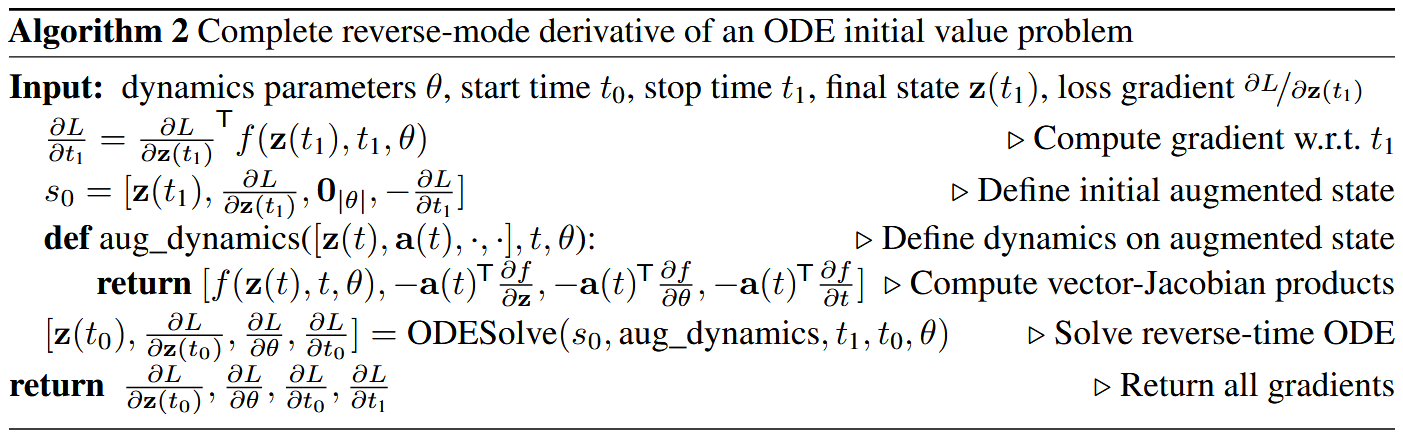
\includegraphics[width=0.95\textwidth]{figures/Algorithm.png}
    \end{center}
    % \caption{}\label{fig:}
  \end{figure}
\end{frame}

\begin{frame}{Replacing Resnet}
  \begin{figure}
    \begin{center}
      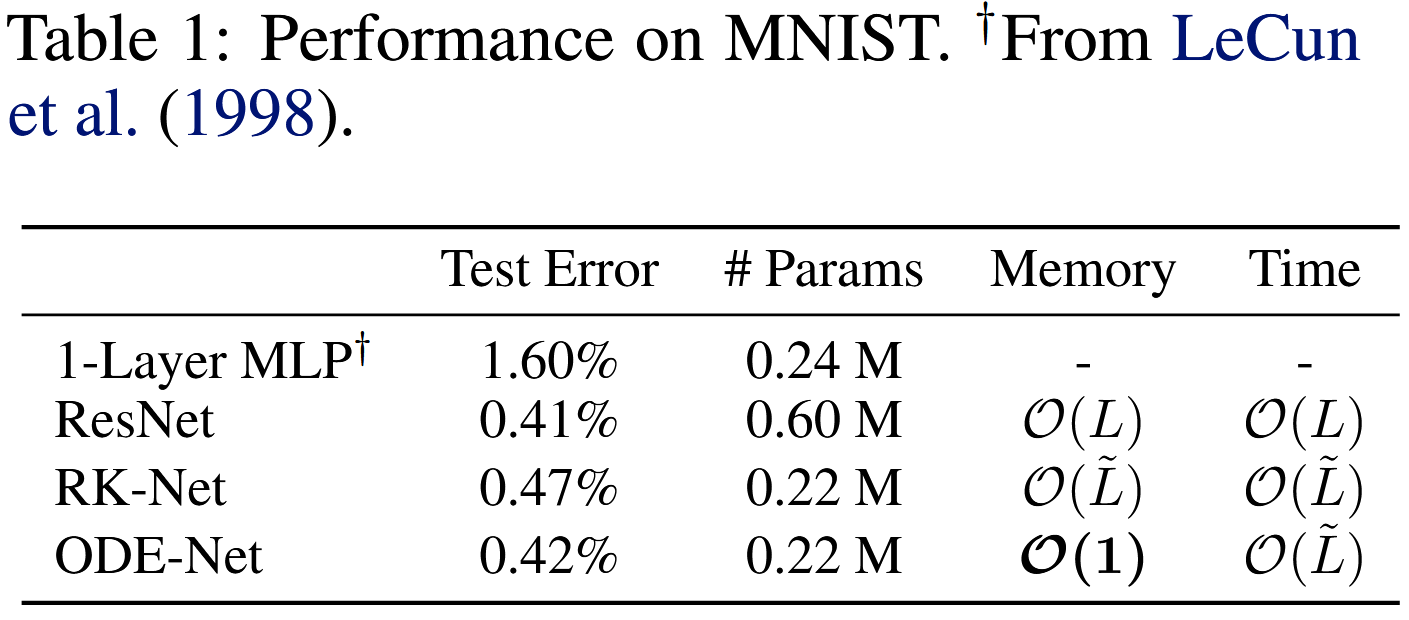
\includegraphics[width=0.5\textwidth]{figures/ODEnet.png}
    \end{center}
    % \caption{}\label{fig:}
  \end{figure}
\end{frame}

\begin{frame}{Continuous Normalizing Flows}
  \begin{gather*}
    \textbf{\textrm{z}}_1 = f(\textbf{\textrm{z}}_0) \Longrightarrow \log p(\textbf{\textrm{z}}_0) 
    - \log \left|\det \frac{\partial f}{\partial \textbf{\textrm{z}}_0}\right| \\
    \Downarrow \\
    \frac{\partial\log p(\textbf{\textrm{z}}(t))}{\partial t}=-\textrm{tr}\left(\frac{\textrm{d}f}
    {\textrm{d}\textbf{\textrm{z}}(t)}\right)
  \end{gather*}
\end{frame}

\begin{frame}{A Generative Lantent Function Time-series Model}
  
\end{frame}

\begin{frame}{Acknowledgement}
  \begin{center}
    \textcolor{gray}{\Huge{\centerline{\calligra{Thank you!}}}}
  \end{center}
\end{frame}

\end{document}
